% This is how you write a comment in Latex

\documentclass[journal]{IEEEtran}

%If you need only single column, use this one:
%\documentclass[journal, onecolumn]{IEEEtran}

%% I have provided the IEEEtran.cls, IEEEtran.sty IEEEtran.bst style
%% files in this directory.  

%% If the above command does not work if your system does not have the
%% IEEE transactions styles installed, then use the following 

%\documentclass[11pt]{article}


% This package is used to write algorithms (see Buchberger's algorithm
% in the text). File algorithm2e.sty included in the directory
\usepackage[ruled]{algorithm2e}
%%for algorithm2e package, label has to be following caption in the same line!!!
\renewcommand{\algorithmcfname}{ALGORITHM}
\SetAlFnt{\small}
\SetAlCapFnt{\small}
\SetAlCapNameFnt{\small}
\SetAlCapHSkip{0pt}
\IncMargin{-\parindent}


% These packages will help you with Math and Figures
\usepackage{helvet}
\usepackage{enumerate}
\usepackage{amsmath}
\usepackage{amsfonts}
\usepackage{graphicx}
\usepackage{multirow}
\usepackage{subfig}
\usepackage{comment}
\usepackage{mathtools}
%\usepackage{algorithm}
%%indent in algorithm


\setcounter{page}{1}


% New command for the table notes.
\def\tabnote#1{{\small{#1}}}

% New command for the line spacing.
\newcommand{\ls}[1]
    {\dimen0=\fontdimen6\the\font
     \lineskip=#1\dimen0
     \advance\lineskip.5\fontdimen5\the\font
     \advance\lineskip-\dimen0
     \lineskiplimit=.9\lineskip
     \baselineskip=\lineskip
     \advance\baselineskip\dimen0
     \normallineskip\lineskip
     \normallineskiplimit\lineskiplimit
     \normalbaselineskip\baselineskip
     \ignorespaces
    }




\newtheorem{Algorithm}{Algorithm}[section]
\newtheorem{Definition}{Definition}[section]
\newtheorem{Example}{Example}[section]
\newtheorem{Proposition}{Proposition}[section]
\newtheorem{Lemma}{Lemma}[section]
\newtheorem{Theorem}{Theorem}[section]
\newtheorem{Corollary}{Corollary}[section]
\newtheorem{Proof}{Proof}


%%% These are my macros that I use for math symbols

\newcommand{\B}{{\mathbb{B}}}
\newcommand{\Z}{{\mathbb{Z}}}
\newcommand{\R}{{\mathbb{R}}}
\newcommand{\Q}{{\mathbb{Q}}}
\newcommand{\N}{{\mathbb{N}}}
\newcommand{\C}{{\mathbb{C}}}
\newcommand{\Zn}{{\mathbb{Z}}_{n}}
\newcommand{\Zp}{{\mathbb{Z}}_{p}}
\newcommand{\F}{{\mathbb{F}}}
\newcommand{\Fbar}{{\overline{\mathbb{F}}}}
\newcommand{\Fq}{{\mathbb{F}}_{q}}
\newcommand{\Fqbar}{{\overline{{\mathbb{F}}_q}}}
\newcommand{\Fkk}{{\mathbb{F}}_{2^k}}
\newcommand{\Zkk}{{\mathbb{Z}}_{2^k}}
\newcommand{\Fkkx}[1][x]{\ensuremath{\mathbb{F}}_{2^k}[#1]\xspace}
\newcommand{\Grobner}{Gr\"{o}bner\xspace}
\newcommand{\bi}{\begin{itemize}}
\newcommand{\ei}{\end{itemize}}

\newcommand{\idealj}{{J = \langle f_1, \dots, f_s\rangle}}
\newcommand{\idealg}{{J = \langle g_1, \dots, g_t\rangle}}
\newcommand{\vfqj}{{V_{\Fq}(J)}}
\newcommand{\vfkkj}{{V_{\Fkk}(J)}}


\newcommand{\debug}[1]{\textcolor{red}{[ #1 ]}}

%%set spacing between table columns
\setlength{\tabcolsep}{3pt}

%% for larger matrices
\setcounter{MaxMatrixCols}{15}

%\IEEEoverridecommandlockouts

\begin{document}


%Page header
\markboth{Kalla wrote this document}{Prof. Kalla is the best}

%% \title{\large{\textsc{Formal Verification of Galois Field Arithmetic
%%       Circuits using Computer Algebra Techniques }}}  

\title{Engineers Know How to Put Math to Work}
\author{Student 1, Student 2\\
Department of  Electrical and Computer Eng.\\
University of Utah, Salt Lake City, UT-84112\\\{myemail\}@utah.edu }


\maketitle


%%%%%%%%%%%%%% Include your files here in separate files 
\begin{abstract}
Galois fields have wide applications in the VLSI domain. This paper
describes a new approach to verify VLSI implementations of digital
circuits using Gr\"obner basis methods. The verification problem is
modeled as proving the infeasibility of a miter using Hilbert's
Nullstellensatz. Buchberger's algorithm is then applied to reason
about the variety of ideals corresponding to the VLSI
circuits. Experiments demonstrate the superiority of this method
against contemporary SAT-based verification when applied to datapath
dominated applications. 
\end{abstract}

\section{Introduction}

To compile this document, run the following commands: 

\begin{verbatim}
prompt> latex latex-for-class
prompt> bibtex latex-for-class
prompt> latex latex-for-class
prompt> latex latex-for-class
prompt> dvips -o latex-for-class.ps latex-for-class
prompt> ps2pdf latex-for-class.ps
\end{verbatim}

This will create the latex-for-class.pdf file. You have to run latex a
couple of times to get cross-references resolved. 

\subsection{Math Symbols}

This is {\it italics}, {\bf bold font}. This is how we use math mode:

\begin{align}
A = a_0 + a_1 \alpha + a_2 \alpha^2 = \sum _{i=0}^{2} a_i \cdot \alpha^i
\end{align}

This is also how to use in-line math mode: $\F, \R, \Q, \C, \Fq,
\Fkk$, based on my macros.

Let $ \idealj = \idealg \subseteq \Fq[x_1, \dots, x_n]$ and let $V(J)$
denote the variety $V$ of ideal $J$. Actually, since variety is needed
over $\Fq$ itself, use $\vfqj$.

This is how you write an algorithm and refer to it as
Alg. \ref{alg:gb}, see the caption below the algorithm description in
the intro.tex file.

\begin{algorithm}[hbt]
\SetAlgoNoLine
 \KwIn{$F = \{f_1, \dots, f_s\}$}
 \KwOut{$G = \{g_1,\dots ,g_t\}$\\} %, a Gr\"{o}bner basis
  $G:= F$\;
  \Repeat{$G = G'$}
  {
  	$G' := G$\;
  	\For{ each pair $\{f, g\}, f \neq g$ in $G'$} 
	{
		$Spoly(f, g) \stackrel{G'}{\textstyle\longrightarrow}_+r$ \;
		\If{$r \neq 0$}
		{
			$G:= G \cup \{r\}$ \;
		}
	}
   }
\caption {Buchberger's Algorithm}
\label{alg:gb}
\end{algorithm}

This is how you write the polynomial reduction of $f \pmod{ G}: f
\xrightarrow{g_1, \dots, g_t} _+ r$ where $G = \{g_1, \dots,
g_t\}$. Also, there are many ways to write a matrix, two of them are: 

\[
M = \begin{pmatrix*}[l]
 & x^2y & y^3 & y^2 & y\\
f_4 & \frac{1}{3} & \frac{1}{2} & 0 & 0 \\
yf_1 & 2 &0 & 1 & 0 \\
yf_3 & 0 & 4 & 0 & -1
\end{pmatrix*}
\]

\[
M = \bordermatrix{
~ & x^2y & y^3 & y^2 & 1\cr
f_4 & \frac{1}{3} & \frac{1}{2} & 0 & 0 \cr
yf_1 & 2 &0 & 1 & 0 \cr
f_3 & 0 & 4 & 0 & -1 \cr
}
\]

Now, reducing $M$ to a row echelon form using Gaussian elimination gives:
\[
M = \bordermatrix{
~ & x^2y & y^3 & y^2 & 1\cr
f_4 & \frac{1}{3} & \frac{1}{2} & 0 & 0 \cr 
h = f_4 - \frac{1}{6}yf_1 & 0 &\frac{1}{3}  & -\frac{1}{6} & 0 \cr 
r = h - \frac{1}{8}f_3 & 0 & 0 & -\frac{1}{6} & \frac{1}{8} \cr 
}
\]


This is how you provide citation for a journal paper \cite{ted_tcomp},
conference paper \cite{shekhar:fmcad06}, book \cite{ideals:book} or a
PhD thesis \cite{buchberger_thesis}.  

\begin{Theorem}
This theorem states that Prof. Kalla is indeed the best.
\end{Theorem}

\begin{Proof}
The proof is trivial.
\end{Proof}

\begin{Corollary}
No one is better than Prof. Kalla.
\end{Corollary}

Finally, this is how you include a figure as shown in Fig. \ref{fig:ckt}. 

\begin{figure}[hbt]
\centering
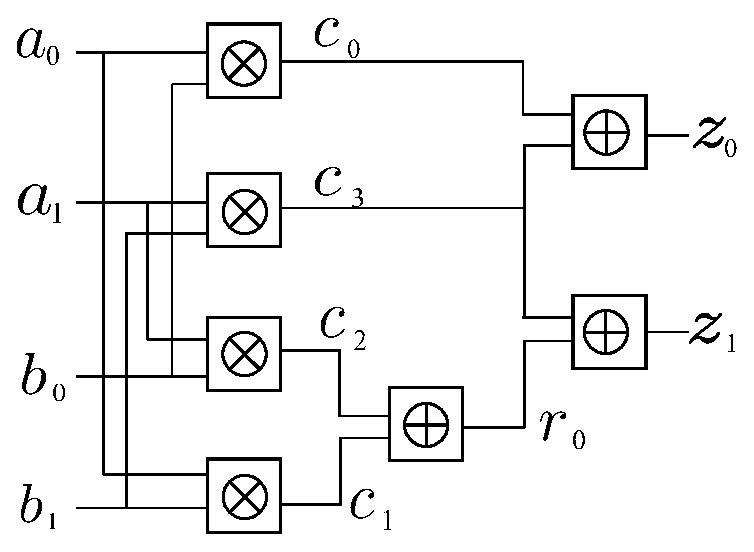
\includegraphics[scale=0.5]{2bitmultiplier.eps}
\caption{This is a figure}
\label{fig:ckt}
\end{figure}
\section{Experimental Results}

When you complete your project, your results should compare like
this. If not, all of you will fail the course. As shown in Table
\ref{tab:ourmas}, both {\sc Singular} and our 
$F4$ approach can verify the correctness of up to 
$163$-bit Mastrovito multipliers -- corresponding to the practical
NIST-specified Galois field ${\mathbb{F}}_{2^{163}}$.  However, our
$F4$-style approach is almost $2.5X$ faster. 

\begin{table}[htb!]
\begin{center}
\caption{ Runtime for verifying bug-free and buggy Mastrovito
  multipliers using our approach. TO = timeout of 10hrs. Time is given
  in seconds.}  
\label{tab:ourmas}
\begin{tabular}{|c||c|c|c|c|c|c|} \hline 
Operand size $k$: & 32 &  64 & 96 & 128  &160 &163\\
\hline
\#variables   &$1155$ 		&$4355$ 	&$9603$ 	&$16899$ 	&$26243$ 	&$27224$ \\
\hline
\#polynomials &$1091$ 		&$4227$ 	&$9411$ 	&$16643$ 	&$25923$ 	&$26989$ \\
\hline
\#terms        &$7169$ 	&$28673$ 	&$64513$ 	&$114689$ 	&$179201$ 	&$185984$ \\
\hline
\hline
Bug-free (Singular) &$1.41$ 		&$112.13$ 	&$758.82$ 	&$3054$ 	&$9361$ 	&$16170$ \\
\hline
Bug-free ($F_4$) &$0.83$ 		&$39.23$ 	&$243.16$ 	&$1138$ 	&$3496$ 	&$6537$ \\
\hline \hline
Bugs (Singular) &$1.43$		&$114.86$ 	&$788.65$ 	&$3061$  	&$9384$ 	&$16368$\\
\hline
Bugs ($F_4$)  &$0.84$		&$40.01$ 	&$249.84$ 	&$1152$  	&$3530$ 	&$6592$\\
\hline
\end{tabular}
\end{center}
\end{table}



%%%%%%%%%%%%%%%%%%%% The bibliography %%%%%%%%%%%%%%%%%%%%%%%%%%%%
%% I am providing IEEE style bibliography formatting through the file IEEEtran.bst file
\bibliographystyle{IEEEtran}
\bibliography{ref}

\end{document}

%%%%%%%%%%%%%%%%%%%%%%%%%%%  End of IEEEsample.tex  %%%%%%%%%%%%%%%%%%%%%%%%%%%
